\documentclass[11pt]{article}

\usepackage[T1]{fontenc}
\usepackage{lmodern}
\usepackage[margin=1in]{geometry}
\usepackage{graphicx}
\usepackage{booktabs}
\usepackage{xcolor}
\usepackage{listings}
\usepackage{caption}
\usepackage{float}
\usepackage{enumitem}
\usepackage[hidelinks,colorlinks=true,linkcolor=blue!55!black,urlcolor=blue!55!black]{hyperref}

\graphicspath{{figures/}}
\setlength{\parskip}{0.5em}
\setlength{\parindent}{0pt}
\setlength{\emergencystretch}{3em}
\sloppy
\captionsetup{font=small,labelfont=bf}

\definecolor{codebg}{gray}{0.95}
\lstdefinestyle{mono}{
  basicstyle=\ttfamily\footnotesize,
  breaklines=true,
  breakatwhitespace=false,
  columns=fullflexible,
  keepspaces=true,
  frame=single,
  framesep=4pt,
  rulecolor=\color{gray!55},
  backgroundcolor=\color{codebg},
  xleftmargin=4pt,
  xrightmargin=4pt,
}
\lstset{style=mono}

% Convenience for a full-width captioned figure.
\newcommand{\figurewide}[3]{%
  \begin{figure}[H]\centering
    \includegraphics[width=\linewidth]{#1}
    \caption{#2}\label{#3}
  \end{figure}}

\begin{document}

\begin{titlepage}
\centering
\vspace*{1.5cm}
{\LARGE\bfseries Indirect Denial-of-Service via\\[2pt] Health-Check Manipulation in Docker Swarm\par}
\vspace{0.6cm}
{\large A Restart-Storm Availability Attack on Containerized Microservices\\ --- and its Detection and Mitigation\par}
\vspace{1.4cm}

\begin{tabular}{rl}
\textbf{Course} & Information Security (CEP-2026)\\[3pt]
\textbf{Department} & Software Engineering, NED University of\\
                   & Engineering \& Technology\\[3pt]
\textbf{Instructor} & Miss Sheerina\\[3pt]
\textbf{Group} & B14\\
\end{tabular}

\vspace{1.0cm}
{\large\bfseries Group Members\par}
\vspace{0.3cm}
\begin{tabular}{ll}
\toprule
\textbf{Name} & \textbf{Reg. No.}\\
\midrule
Muhammad Abdullah Khan & SE-23061\\
Furqanullah & SE-23063\\
Masroor Hassan & SE-23064\\
Haris Masood & SE-23088\\
Muhammad Huzaifa Hassan & SE-23089\\
Muhammad Rafay & SE-23100\\
\bottomrule
\end{tabular}

\vfill
{\small Single-node Docker Swarm testbed. All metrics measured on the authors' own host.\par}
\end{titlepage}

\tableofcontents
\newpage

\section*{Abstract}
\addcontentsline{toc}{section}{Abstract}

In Docker Swarm, a single \texttt{HEALTHCHECK} drives \emph{two} independent
decisions at once: whether a task receives traffic, and whether a task is
restarted. When that health-check depends on an external resource such as a
database, an attacker who merely \emph{slows the dependency} --- without ever
touching the victim container --- makes the health-check time out. Swarm's
\texttt{restart\_policy}, behaving exactly as designed, then kills and recreates
the task again and again: a \textbf{restart storm} that takes the service
offline even though the application code is perfectly functional.

We reproduced this attack in a controlled single-node Swarm testbed, built a
real-time detector that identifies the storm and names its cause, and applied a
mitigation that separates process liveness from dependency health. Measured
before and after, the same attack drops \texttt{/work} availability to
\textbf{21\%} with \textbf{2} forced restarts on the vulnerable stack, but leaves
availability at \textbf{100\%} with \textbf{0} restarts on the mitigated stack.
The detector raises its first alert \textbf{17.7\,s} after the attack begins and
correctly stays silent when no storm occurs.

\section{Introduction and Motivation}

Container orchestrators health-check every service and act on the result. In
Docker Swarm the same probe is overloaded: a failing probe simultaneously
removes the task from the load-balancer rotation \emph{and} feeds the restart
decision. This coupling is convenient, widely taught, and ships by default ---
the canonical tutorial health-check pings the database. It is also the root of
the vulnerability studied here.

The insight of this project is that \textbf{availability can be destroyed
without attacking the victim at all.} The application process can be healthy,
answering real requests correctly, and still be killed repeatedly by its own
orchestrator because a \emph{dependency} it probes has been slowed. The
attacker's capability required is minimal: the ability to add latency to one
network path.

\section{Problem Description --- The Indirect DoS and the Restart Storm}

The failure chain has five stages and never touches the victim container:

\begin{enumerate}[nosep]
\item The attacker slows a dependency (here, the database path) so responses
  take longer than the health-check timeout.
\item The service's \texttt{/health} probe performs a database round-trip and
  times out.
\item After the configured retries, Docker marks the container
  \textbf{unhealthy}.
\item Swarm treats the unhealthy task as failed and, under a
  \texttt{restart\_policy} with no \texttt{max\_attempts}, terminates and
  recreates it.
\item The replacement task boots, fails the same dependency-coupled probe, and
  is killed again --- a continuous terminate-and-restart cycle (the
  \emph{restart storm}). The service is unavailable for the duration.
\end{enumerate}

The defining fingerprint --- the \textbf{signature signal} --- is a
\emph{divergence}: the application keeps succeeding at real work while the
health-check keeps failing. In our captured logs the application logs
\texttt{WORK ok} right up to each \texttt{HEALTH fail \ldots\ timeout expired},
proving the code is alive while Swarm kills it.

\section{Relevance to Containerized Environments}

This is specifically an \emph{orchestration} problem, not a generic web-app bug:

\begin{itemize}[nosep]
\item \textbf{Orchestrator coupling.} Swarm's single health-check drives both
  routing and restart. One failed probe triggers two corrective actions at
  once; there is no separation of concerns.
\item \textbf{\texttt{restart\_policy} amplification.} Auto-restart converts a
  transient dependency blip into a sustained outage. The orchestrator actively
  degrades availability \emph{while trying to restore it} --- a self-inflicted
  DoS.
\item \textbf{Microservice blast radius.} Every service whose health-check
  touches a degraded dependency fails together; one slow database can collapse a
  whole request path in seconds.
\item \textbf{Default-config exposure.} The vulnerable pattern (health-check
  pings the database) is the documented ``best practice'' in tutorials and Helm
  charts, so the risky configuration is shipped by default.
\end{itemize}

In a monolith where health and routing are decoupled, this class of risk is
absent. The orchestrator is what turns a \emph{dependency failure} into an
\emph{availability failure}.

\section{Threat Model}

\begin{itemize}[nosep]
\item \textbf{Attacker goal:} deny availability of a target service.
\item \textbf{Attacker capability:} inject latency into the network path between
  the service and one of its dependencies (modelled here with a latency
  injector). No code execution, no credentials, and no access to the victim
  container are required.
\item \textbf{What the attacker never does:} touch, exploit, or even reach the
  victim web container. Only the dependency path is slowed.
\item \textbf{Assumptions:} the service runs a dependency-coupled health-check
  (the default pattern) and a \texttt{restart\_policy} without a bounded
  \texttt{max\_attempts}.
\item \textbf{Out of scope:} classic volumetric/network DDoS, host compromise,
  multi-node cluster effects. The single-node testbed reproduces the same
  orchestrator behaviour without them.
\end{itemize}

\section{Testbed Design}

A single-host Docker Swarm (\texttt{docker swarm init}, one Ready node) runs
three services on one overlay network: \texttt{web} (the Flask victim service),
\texttt{db} (\texttt{postgres:16}, the dependency), and \texttt{toxiproxy}
(the latency injector between \texttt{web} and \texttt{db}).

The web app exposes deliberately separated endpoints: \texttt{/work} (real work,
never touches the database), \texttt{/health} (the \emph{vulnerable} probe: a
database round-trip through Toxiproxy), \texttt{/healthz} (the \emph{mitigated}
local-only liveness probe), \texttt{/ready} (database-dependent readiness,
guarded by a circuit breaker), and \texttt{/metrics} (Prometheus metrics). The
application reaches the database \emph{only} through Toxiproxy, so the attack can
slow the database path without touching \texttt{web}. Two stack files differ
only in the two settings that matter: \texttt{vulnerable.yml} (health-check
probes \texttt{/health}; \texttt{restart\_policy} has no \texttt{max\_attempts})
and \texttt{mitigated.yml} (health-check probes \texttt{/healthz};
\texttt{restart\_policy} adds \texttt{max\_attempts: 3} and a \texttt{window}).

\figurewide{term_reset_vuln.png}{Clean start: \texttt{reset.ps1} brings up the
vulnerable stack plus the Prometheus/Grafana dashboard on a single Swarm node;
the web service reaches \emph{healthy} and all endpoints are listed.}{fig:reset}

\figurewide{grafana_baseline_top.png}{Baseline (no attack) on the live Grafana
dashboard: the web task is continuously UP, the restart count is 0, and the
request/health panels are steady.}{fig:baseline}

\section{Attack Demonstration --- Method and Evidence}

\textbf{Method.} The attack is a single action: add a latency \emph{toxic}
(5000\,ms) to the Toxiproxy route via its control API, so database replies
exceed the health-check timeout. A load generator samples \texttt{/work}
throughout, and \texttt{docker stack ps} plus the service logs are captured.

\textbf{Evidence.} During the attack, Swarm repeatedly kills the healthy task.
The task history states the cause explicitly --- \texttt{"non-zero exit (137):
dockerexec: unhealthy container"} (Figure~\ref{fig:storm}).

\figurewide{stackps_storm.png}{The restart storm in \texttt{docker stack ps app}:
a replacement \texttt{app\_web} task is \emph{Starting} while the previous one is
\emph{Shutdown / Failed} with \texttt{"non-zero exit (137): dockerexec:
unhealthy container"}. Swarm is killing a process that is in fact
alive.}{fig:storm}

The \textbf{signature signal} is visible in the application log: real work
succeeds (\texttt{WORK ok \ldots\ 200}) while the health-check fails on a
database timeout (\texttt{HEALTH fail \ldots\ 503 \ldots\ timeout expired}),
interleaved on the same running task (Figure~\ref{fig:signature}).

\figurewide{log_signature_signal.png}{Signature signal in the web service log:
\texttt{/work} returns 200 while \texttt{/health} returns 503 with a Toxiproxy
timeout. The application code is healthy; only the dependency-coupled probe
fails.}{fig:signature}

On the live dashboard the ``web UP'' panel shows a red gap for the period the
task is down, and the health-check \emph{fail} series rises
(Figure~\ref{fig:redgap}); once Swarm has replaced the task, the restart counter
registers the event (Figure~\ref{fig:restartcount}).

\figurewide{grafana_attack_redgap.png}{Grafana during the attack: the ``web
task UP'' panel shows a red down-period (the restart gap), and the health-check
panel begins recording failures.}{fig:redgap}

\figurewide{grafana_restart_count.png}{The restart is detected without cAdvisor:
\texttt{changes(process\_start\_time\_seconds)} increments the ``Web restarts''
stat as Swarm recreates the task.}{fig:restartcount}

When the toxic is removed, the service recovers on its own
(Figure~\ref{fig:recovery}). The victim container was never attacked --- only
the database path was slowed.

\figurewide{term_recovery_servicels.png}{Recovery: after
\texttt{attack.ps1 off}, \texttt{docker service ls} shows every service back at
\texttt{1/1}.}{fig:recovery}

\section{Detection}

\texttt{detector/monitor.py} (Docker SDK for Python) watches three signals in
real time and writes alerts to \texttt{results/alerts.log}:

\begin{enumerate}[nosep]
\item \textbf{Health events.} Streams container \texttt{health\_status} events
  and counts repeated \texttt{unhealthy} transitions in a sliding window
  (health flapping).
\item \textbf{Restart frequency.} Polls the service tasks and counts restarts in
  a sliding window, alerting past a configurable threshold.
\item \textbf{Signature signal.} When health fails, it probes \texttt{/work}
  \emph{inside} the container (via \texttt{docker exec}, bypassing the de-routed
  ingress mesh). A 200 proves the application is alive, so the detector reports
  an \textbf{indirect DoS} caused by dependency latency --- not a crash.
\end{enumerate}

The detector raised its first alert \textbf{17.7\,s} after the attack began and,
on the mitigated stack, correctly produced \textbf{no alerts} --- there was no
storm to detect. Thresholds live in a config block so the team can tune them.

\figurewide{detector_alerts.png}{Live detector output: \texttt{INDIRECT-DOS},
\texttt{HEALTH-FLAP} and \texttt{RESTART-STORM} alerts, each naming the cause as
dependency latency rather than an application crash.}{fig:detector}

\section{Mitigation}

\textbf{Core fix (required).}
\begin{itemize}[nosep]
\item \textbf{Separate liveness from readiness.} The container
  \texttt{HEALTHCHECK} now probes \texttt{/healthz}, a local-only liveness check
  that does \emph{not} touch the database. A slow dependency can no longer fail
  the health-check, so Swarm no longer kills a healthy container.
  \texttt{/ready} keeps the database check for \emph{routing} decisions only.
\item \textbf{Tune the restart policy.} \texttt{restart\_policy} gains
  \texttt{max\_attempts: 3} and a \texttt{window: 60s}, so even a genuine failure
  cannot become an unbounded storm.
\end{itemize}

\textbf{Defence-in-depth (optional, implemented).}
\begin{itemize}[nosep]
\item \textbf{Circuit breaker} around the database call: after repeated slow
  calls the breaker opens and \texttt{/ready} fails fast
  ($\approx$10\,ms) instead of hanging for the full timeout on every request.
\item \textbf{Reverse proxy (HAProxy)} that health-checks \texttt{/ready} and
  de-routes a slow instance \emph{without killing it}. Captured proof under
  latency: \texttt{/healthz} $\to$ 200, \texttt{/ready} $\to$ 503,
  \texttt{/work} $\to$ 200, and the container is never killed.
\end{itemize}

Switching to the mitigated stack is a single command
(Figure~\ref{fig:fix}); under the \emph{same} attack, \texttt{docker stack ps}
shows no killed tasks at all (Figure~\ref{fig:nokills}).

\figurewide{term_fix_mitigated.png}{\texttt{fix.ps1} redeploys the mitigated
stack (liveness-only health-check + bounded restart policy); the web service
comes up healthy.}{fig:fix}

\figurewide{stackps_mitigated_nokills.png}{The same attack on the mitigated stack
(\texttt{iddos-app:fixed}): every task is \emph{Running} with \emph{no}
\texttt{Shutdown/Failed} rows --- the restart storm is gone.}{fig:nokills}

\section{Results}

All three scenarios used the same attack (5000\,ms latency), a 90\,s attack
window, and \texttt{/work} sampled at 5 requests/second.

\begin{table}[H]\centering
\caption{Before/after metrics across the three scenarios.}
\begin{tabular}{llccccc}
\toprule
\textbf{Scenario} & \textbf{Stack} & \textbf{Attack} & \textbf{Avail.} & \textbf{Restarts} & \textbf{MTTR (s)} & \textbf{TTD (s)}\\
\midrule
Baseline & vulnerable & no & 100.0\% & 0 & --- & ---\\
Vulnerable + attack & vulnerable & yes & 21.0\% & 2 & 13.0 & 17.7\\
Mitigated + attack & mitigated & yes & 100.0\% & 0 & 0.2 & ---\\
\bottomrule
\end{tabular}
\end{table}

\emph{Metrics.} \textbf{Availability} = share of \texttt{/work} requests
returning 200; \textbf{Restarts} = web task restarts in the attack window;
\textbf{MTTR} = seconds from the toxic being removed to the web service becoming
healthy again; \textbf{TTD} (time-to-detection) = seconds from attack start to
the detector's first alert (``---'' = no alert, i.e.\ no storm to detect).

\begin{figure}[H]\centering
  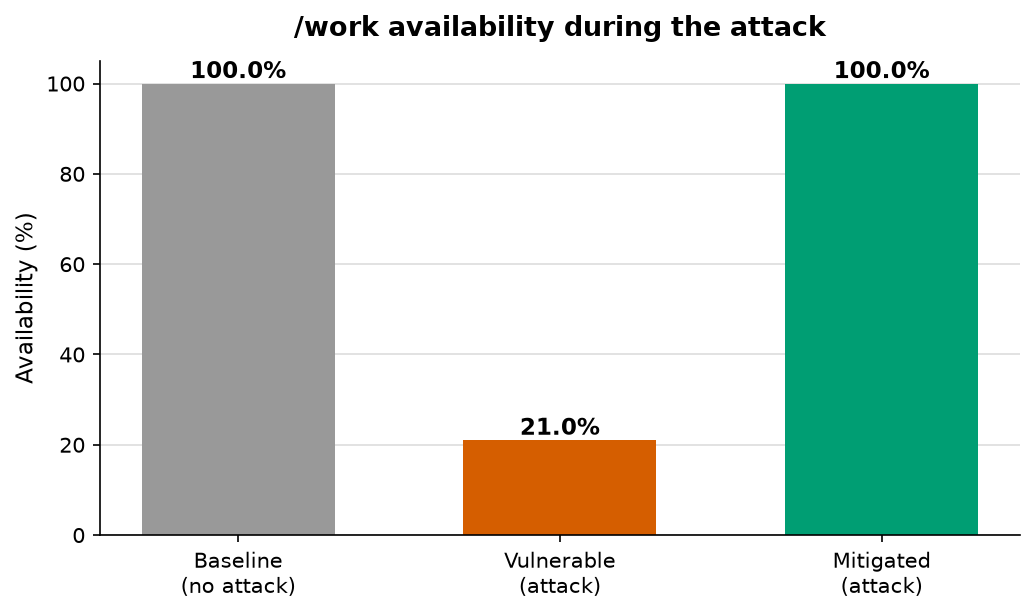
\includegraphics[width=0.78\linewidth]{fig_availability.png}
  \caption{\texttt{/work} availability during the attack: 100\% baseline,
  21\% on the vulnerable stack, 100\% on the mitigated stack.}
  \label{fig:avail}
\end{figure}

\begin{figure}[H]\centering
  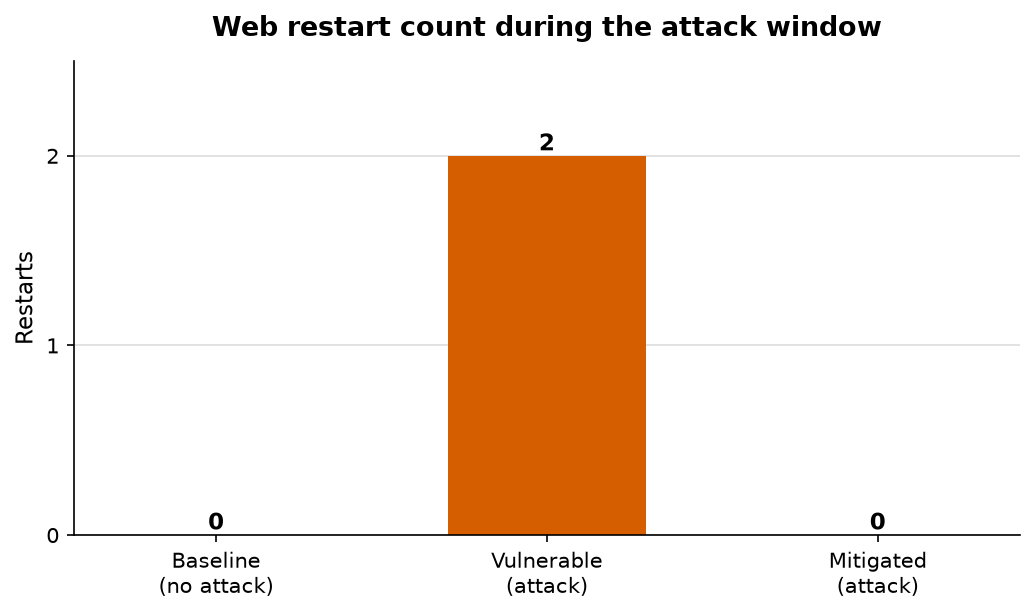
\includegraphics[width=0.78\linewidth]{fig_restarts.png}
  \caption{Web restart count during the attack window: 2 on the vulnerable
  stack, 0 on the mitigated stack.}
  \label{fig:restarts}
\end{figure}

\figurewide{grafana_mitigated_flat.png}{The mitigated stack under the same
attack on the live dashboard: the web task stays UP and the restart count holds
at 0.}{fig:mitflat}

\textbf{Reading the results.} On the vulnerable stack the attack is devastating:
availability falls to roughly one-fifth and the orchestrator forces repeated
restarts. On the mitigated stack the \emph{same} attack is a non-event:
availability holds at 100\%, no restarts occur, and recovery is immediate. This
meets every acceptance target set for the project (availability $\ge$ 95\%,
restarts low/zero, short MTTR, detection $\le$ 30\,s).

\section{Conclusion and Future Work}

An orchestrator feature intended to improve availability --- automatic restart
on a failed health-check --- becomes an availability \emph{weapon} when the
health-check is coupled to an external dependency. The attack needs no exploit on
the victim; it only slows a dependency. The fix is architectural and
inexpensive: \textbf{separate process liveness from dependency health} and
\textbf{bound the restart policy}. Our measurements show the mitigation
neutralises the attack completely in this testbed.

\textbf{Future work.} Extend to a multi-node cluster and multiple dependent
services to observe cascade/blast-radius effects; compare Swarm's behaviour with
Kubernetes liveness/readiness/startup probes; add automated alerting rules in
Prometheus; and study adaptive attackers that keep latency just below the
detection threshold.

\section{References}

\textbf{Container orchestration}
\begin{enumerate}[nosep]
\item Docker Inc. (2024). \emph{Configure healthchecks in Docker Swarm.} Docker Documentation.
\item Burns, B., Grant, B., Oppenheimer, D., Brewer, E., \& Wilkes, J. (2016). \emph{Borg, Omega, and Kubernetes.} ACM Queue, 14(1).
\end{enumerate}

\textbf{DoS / availability attacks}
\begin{enumerate}[nosep,start=3]
\item Carl, G., Kesidis, G., Brooks, R. R., \& Rai, S. (2006). \emph{Denial-of-Service Attack-Detection Techniques.} IEEE Internet Computing, 10(1).
\item Peng, T., Leckie, C., \& Ramamohanarao, K. (2007). \emph{Survey of network-based defense mechanisms countering the DoS and DDoS problems.} ACM Computing Surveys, 39(1).
\end{enumerate}

\textbf{Microservice \& cascade failures}
\begin{enumerate}[nosep,start=5]
\item Newman, S. (2021). \emph{Building Microservices: Designing Fine-Grained Systems}, 2nd ed. O'Reilly Media.
\item Richardson, C. (2019). \emph{Microservices Patterns.} Manning Publications. (Chapter on circuit breakers.)
\item Aceto, G., Botta, A., Marchetta, P., Persico, V., \& Pescap\`{e}, A. (2018). \emph{Cloud monitoring: A survey.} Computer Networks, 57(9).
\end{enumerate}

\appendix
\section{Reproducing the Results}

From the \texttt{iddos-swarm/} directory (see \texttt{README.md} and
\texttt{demo/runbook.md} for detail):

\begin{lstlisting}
# build images
docker build -t iddos-app:vuln app/
docker build -f app/Dockerfile.fixed -t iddos-app:fixed app/

# full measured comparison (writes results/metrics.csv + charts)
python load/measure.py
python load/make_charts.py

# live demo (PowerShell on Windows)
.\demo\reset.ps1          # vulnerable stack + dashboard (http://localhost:3000)
.\demo\attack.ps1         # start the attack;  .\demo\attack.ps1 off to stop
.\demo\fix.ps1            # switch to the mitigated stack
\end{lstlisting}

\section{Additional Dashboard Views}

\figurewide{grafana_baseline_bottom.png}{Baseline dashboard (lower panels):
\texttt{/work} request rate, health-check pass/fail, and DB probe
latency.}{fig:basebottom}

\figurewide{grafana_attack_bottom.png}{During the attack (lower panels): the
health-check \emph{fail} series appears and DB probe latency spikes toward the
injected delay.}{fig:attackbottom}

\figurewide{term_teardown.png}{Teardown: \texttt{attack.ps1 off} followed by
\texttt{docker stack rm app} removes all services, configs and the overlay
network.}{fig:teardown}

\end{document}
